\documentclass[11pt]{article}   %Needed for every document
\usepackage[margin=0.75in]{geometry}           %Going to help get paper size right
\geometry{letterpaper}          %Normal paper
\usepackage{multicol}
\usepackage{graphicx,epsfig}    %Graphics packages and pictures
\usepackage{amssymb}            %Package for symbols

\usepackage{epstopdf}
\usepackage{color}
\graphicspath{ {Figures/} }
\DeclareGraphicsRule{.tif}{png}{.png}{`convert #1 `dirname #1`/`basename #1 .tif`.png}  %Need for pictures
\newcommand{\ignore}[1]{} %used to make inline comments
\definecolor{gray}{rgb}{0.1, 0.1, 0.1}
\newcommand{\gray}[1]{\colorbox{gray}{#1}}
\usepackage[utf8]{inputenc}
\usepackage[most]{tcolorbox}
\usepackage{hyperref}
\usepackage{listings}

\title{JSON & Webscraping}
\author{Steven Walton\\     %Note that we don't close until after address to keep in title format.
\textit{PS 232 Computational Methods}\\
\textit{Department of Physics}\\
\textit{Embry-Riddle Aeronautical University}\\
\textit{Prescott, AZ   86301}}

\tcbset{
       frame code={}
       center title,
       left=0pt,
       right=0pt,
       top=0pt,
       bottom=0pt,
       colback=gray!70,
       colframe=white,
       width=\dimexpr\textwidth\relax,
       enlarge left by=0mm,
       boxsep=5pt,
       arc=0pt,outer arc=0pt,
       }

\begin{document}

\maketitle
\section*{What is JSON}
JSON is short for JavaScript Object Notation.  It is an open standard format for human readable transmission of data objects.  JSON has six basic types; numbers, string, booleans, arrays, objects, and null.  To get a basic feel of 
what JSON looks like, here is an example:
\begin{tcolorbox}
   \begin{lstlisting}
   {
      ``firstName'': ``John'',
      ``lastName'': ``Smith'',
      ``isAlive'': true,
      ``age'': 25,
      ``height_cm'': 167.6,
      ``address'': {
         ``streetAddress'': ``21 Jump Street'',
         ``city'': ``New York'',
         ``state'': ``NY'',
         ``postalCode'': 10021-3100``
      },
      ''phoneNumbers``:[
         {
            ''type``: ''home``,
            ''number``: ''212 555-1234``
         },
         {
            ''type``: ''office``,
            ''number``: ''646 555-4567``
         }
      ],
      ''children``: [],
      ''spouse``: null
   }
   \end{lstlisting}
\end{tcolorbox}
If you remember back to when we talked about keywords and dictionaries, lecture 4, this will look extremely similar to you.
\\
Now you are probably asking why you should know this, and what's useful for.  Let's pretend that we want to get something off of the internet, text, data, whatever.  We use JSON. It is the javascript replacement to xml.  The standard is used so that we can extract the needed
information to any language that we want.  We can also do the opposite and output data into JSON notation.  This is really great if you are trying to create a pseudo database.  If you are just going to dump the data right away
then this is a great thing to use.  It is also used a lot for APIs (aka, they aren't going to store data).
If you are writing to the web you should always be using JSON format, and if you are reading from the web you should know how JSON works.  A lot of sites use JSON, including wikipedia.  So if you are interacting with websites in 
any way, this is important to know. I will also suggest that if you are interested in websites and python that you look into the django module (the d is silent).

\subsection*{Some simple examples}
Let's just dive right in and try some simple output with json.  This is a great thing to do from a command line interpreter.  I suggest this for practice over using the compiler.
\begin{tcolorbox}
   \begin{lstlisting}
   import json    # I hope you know you should have to do this

   data = [ ( 'a': 'A', 'b': (2,4), 'c':3.0} ]
   print 'Inside the brackets is what the json type will look like:', 
          json.dumps(data, sort_keys=True, indent=2)
   \end{lstlisting}
\end{tcolorbox}
As you'll notice, this gives the same style as our json example above.  This is great if you are creating a website and need to have data read to the user.  I'm not going to go into how those APIs work, and just stick with python.
\\
Let's work with some Google APIs for the moment.
\subsection*{Google Maps}
So we have to carefully word things when using Google APIs.  Remember to use the maps.googleapis.com address.  So let's try a simple example.  We'll look at the address of the school and export some stuff.
\begin{tcolorbox}
   \begin{lstlisting}
   import pprint as pp
   import urllib2
   import json
   # Assume from now on that I am importing these

   url = ``https://maps.googleapis.com/maps/api/geocode/json?address=
            Embry-Riddle+Aeronautical+University+-+Prescott''
         # Good idea to write the url as a variable for easy access and
         # easy reading
   googleResponse = urllib2.urlopen(url)  # We want to see Google's response
   jsonResponse = json.loads(googleResponse.read())
   pp.pprint(jsonResponse)

   \end{lstlisting}
\end{tcolorbox}
Now we'll notice that the output gives us all the nice information about the campus.  Note that if you don't do pretty print that you'll get a messy output.  But from here we really have all the data that we need.  If we want to
get the longitude and latitude we can do this in two ways.  They are
\begin{tcolorbox}
   \begin{lstlisting}
   # Latitude and longitude in one go with json format still
   jsonResponse['results'][0]['geometry']['location']

   # If we want pure float numbers
   lat = jsonResponse['results'][0]['geometry']['location']['lat']
   lng = jsonResponse['results'][0]['geometry']['location']['lng']
   \end{lstlisting}
\end{tcolorbox}
Note the difference in outputs (if you aren't in command line remember to print these statements out).  But from this information we can actually do some cool things.  Let's create a program that will show us a map of any location we
want, by name.
\\\\
Again, I am not going to show you the entire code, but have included it on the GitHub page under this lecture folder.  You will be able to type any of address that Google recognizes.  Some examples you might want to try are:
\\\\
Embry-Riddle Aeronautical University - Prescott\\
Embry-Riddle Aeronautical University - Prescott King Engineering and Technology Center\\
Golden Gate Bridge\\
China\\
Space Needle\\
My Future\\
77 Massachusetts Ave Cambridge, MA 02139\\
The President\\
22.434335 146.203571\\\\
Have fun with the program.\\

\\
You can make the program a lot simpler if you just want to display the map.  See if you reduce it to do just that.  You should be able to do this in 10 
lines (not including the imports and error handling).  \\

\section*{Webscraping}
Interacting with webpages is a fun and interesting part of programming.  You can get a program to do all kinds of stuff with webpages; from entering forum data, uploading/downloading files, finding links/emails, or interact with a
webpage any way you want.  Only use this power for good.
\\
The simplest example of webscraping is to show you how to gather all the links on a page.  Let's look at all the links that nytimes.com has.
\begin{tcolorbox}
   \begin{lstlisting}
   import requests
   from bs4 import BeautifulSoup as BS

   url = http://nytimes.com      # URL to scrape
   response = requests.get(url)  # Get html response
   data = response.text          # Gets everything in text. Print this
   soup = BS(data)               # Lets BS read the html data

   for links in soup.find_all('a'):
      print link.get('href')     # Finds hyper links and parses them to 
                                 # only the address
   \end{lstlisting}
\end{tcolorbox}
We can also use urllib2 to open the page and then use the read to pass it to BS like we did before, but I thought I'd introduce you to another way of doing this.\\
A challenge I'll give the reader is to store these links into an array and follow through the links recursively.  You'll have to use a loop to append the url's and then follow and collect more.  Be careful with what website you test
this on because some might generate you an endless list.  Remove all doubles so you don't repeat and loop forever.  You may also find internal links and that some links are just relative paths.  Therein lies the challenge :)
\\
\subsection*{BeautifulSoup}
With our small intro to webscraping you are probably most curious about BeautifulSoup.  The purpose of BeautifulSoup is to parse html data, it will even deal with tags that aren't closed!  You can ask BeautifulSoup to find all the
links, like we did above, all the classes, whatever you please.  Working with BeautifulSoup actually requires you to know a little about html.  Unfortunately I'm not going to go into that for you, but I'll give you enough to use 
BeautifulSoup.\\

\begin{centering}
   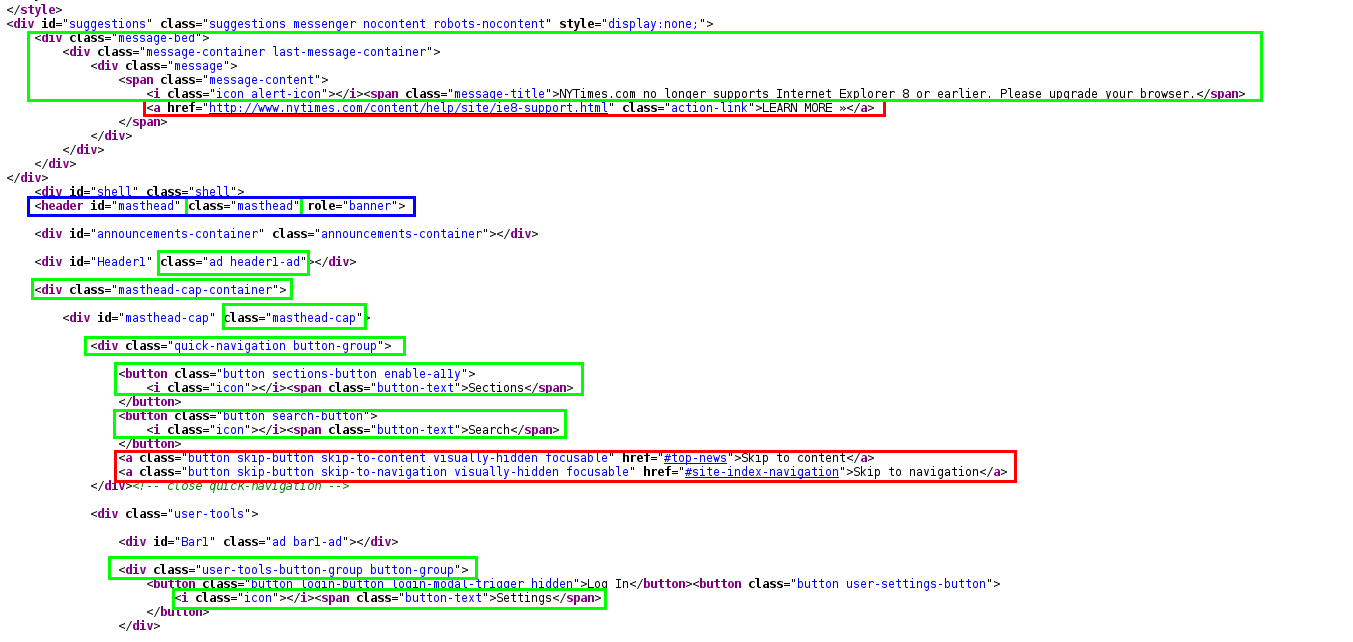
\includegraphics[scale=0.5]{nytimes.png}
\end{centering}
\\
Above we can see a small clipping of the New York Time's home page source code.  In our previous example we looked for 'a' tags and parsed out the href part of the code to get the link (marked with red).  You can also see that I 
highlighted the header in blue and the classes with green.  We can gather all this data and more with BeautifulSoup.  One cool thing we can do with this is gather all the emails listed on a site.  These are usually formatted
<a href=``mailto:username@domain.com''>
\end{document}
